\section{Orbits in an axisymmetric potential}
Considering an axisymmetric potential used as a simple model for a galaxian disk first proposed by Toomre (1964, ApJ):
\begin{equation}
    U(r) = -(1+r^2)^{-1/2}.
\end{equation}

%%%%%%%%%%%%%%%%%%%%%%%%%%%%%%%%%%%%%%%%%%%%%%%%%%%%%%%%%%%%%%%
%=========================SUBSECTION===========================
%%%%%%%%%%%%%%%%%%%%%%%%%%%%%%%%%%%%%%%%%%%%%%%%%%%%%%%%%%%%%%%
\subsection{}
(a) Pick some initial conditions and integrate the orbits using your
orbit integration code. Verify that orbits do not close but precess.
These are sometimes called rosette orbits because of their shape
or tube orbits because the have an inner and outer boundary.

\begin{figure*}
    \centering
    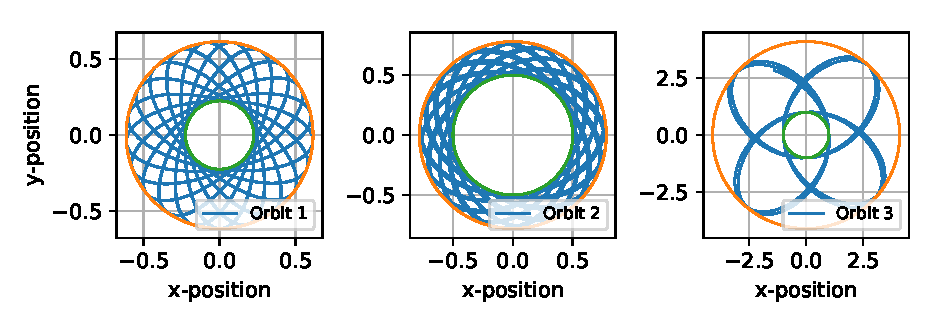
\includegraphics{CodeAndFigures/ToomrePotentialOrbits.pdf}
    \caption{Caption}
    \label{fig:my_label}
\end{figure*}

%%%%%%%%%%%%%%%%%%%%%%%%%%%%%%%%%%%%%%%%%%%%%%%%%%%%%%%%%%%%%%%
%=========================SUBSECTION===========================
%%%%%%%%%%%%%%%%%%%%%%%%%%%%%%%%%%%%%%%%%%%%%%%%%%%%%%%%%%%%%%%
\subsection{}
(b) Compute the energy and angular momentum of your trial orbits
(e.g. using the initial conditions). Compute the inner and outer
radii of the tube (the turning points) using the conserved quantities
and check these values against your direct orbit integration
